\chapter{Instant Insanity Puzzle}

Rishnak was examining the headstones of some of the graves. He saw a headstone with a name Schossow \footnote{ Schossow got a patent for proposing this puzzle in 1899. \url{https://patents.google.com/patent/US646463A/en} }  in a grave. That brought him memories of the puzzle called the Great Tantalizer (also known as Instant Insanity). Schossow's puzzle had card suits (Hearts, Diamonds, Clubs and Spades) marked in each face. Frank Armbruster made a variation of this puzzle with colors instead of suits and that puzzle is called Instant Insanity Puzzle.
Rishnak thought that was a great puzzle to tell Ajur as this puzzle had a nice graph theoretic solution. As Rishnak was thinking, Ajur and Jura walked by. Rishnak told Ajur that he was going to talk about a puzzle which has a short solution using graph theory or a long solution using a search technique. The puzzle consists of four cubes with each face colored as shown in Figure \ref{22p1}. 
\begin{figure}
\begin{center}
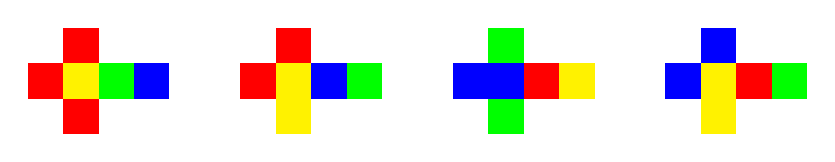
\begin{tikzpicture}
[scale=.9]
%First Cube
\fill [red] (0.0,0.0) rectangle (0.5,0.5);
\fill [yellow] (0.5,0.0) rectangle (1.0,0.5);
\fill [green] (1.0,0.0) rectangle (1.5,0.5);
\fill [blue] (1.5,0.0) rectangle (2.0,0.5);
\fill [red] (0.5,-0.5) rectangle (1.0,0.0);
\fill [red] (0.5,0.5) rectangle (1.0,1.0);
%Second Cube
\fill [red] (3.0,0.0) rectangle (3.5,0.5);
\fill [yellow] (3.5,0.0) rectangle (4.0,0.5);
\fill [blue] (4.0,0.0) rectangle (4.5,0.5);
\fill [green] (4.5,0.0) rectangle (5.0,0.5);
\fill [yellow] (3.5,-0.5) rectangle (4.0,0.0);
\fill [red] (3.5,0.5) rectangle (4.0,1.0);
%Third  Cube
\fill [blue] (6.0,0.0) rectangle (6.5,0.5);
\fill [blue] (6.5,0.0) rectangle (7.0,0.5);
\fill [red] (7.0,0.0) rectangle (7.5,0.5);
\fill [yellow] (7.5,0.0) rectangle (8.0,0.5);
\fill [green] (6.5,-0.5) rectangle (7.0,0.0);
\fill [green] (6.5,0.5) rectangle (7.0,1.0);
%Fourth Cube
\fill [blue] (9.0,0.0) rectangle (9.5,0.5);
\fill [yellow] (9.5,0.0) rectangle (10.0,0.5);
\fill [red] (10.0,0.0) rectangle (10.5,0.5);
\fill [green] (10.5,0.0) rectangle (11.0,0.5);
\fill [yellow] (9.5,-0.5) rectangle (10.0,0.0);
\fill [blue] (9.5,0.5) rectangle (10.0,1.0);
\end{tikzpicture}
\caption{ Four Cubes}\label{22p1}
\end{center}
\end{figure}

The problem is to stack the four cubes vertically (in a column) so that all the cubes in each side (left, right, front and back) have distinct colors.
\begin{figure}
\begin{center}
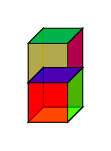
\begin{tikzpicture}
\coordinate (O) at (0,0,0);
\coordinate (A) at (0,0.5,0);
\coordinate (B) at (0,0.5,0.5);
\coordinate (C) at (0,0,0.5);
\coordinate (D) at (0.5,0,0);
\coordinate (E) at (0.5,0.5,0);
\coordinate (F) at (0.5,0.5,0.5);
\coordinate (G) at (0.5,0,0.5);

\draw[black,fill=yellow] (O) -- (C) -- (G) -- (D) -- cycle;% Bottom Face
\draw[black,fill=blue] (O) -- (A) -- (E) -- (D) -- cycle;% Back Face
\draw[black,fill=blue] (O) -- (A) -- (B) -- (C) -- cycle;% Left Face
\draw[black,fill=red,opacity=0.7] (D) -- (E) -- (F) -- (G) --cycle;% Right Face
\draw[black,fill=yellow,opacity=0.7] (C) -- (B) -- (F) -- (G) --cycle;% Front Face
\draw[black,fill=green,opacity=0.7] (A) -- (B) -- (F) -- (E) -- cycle;% Top Face
\coordinate (OO) at (0,-0.5,0);
\coordinate (AA) at (0,0,0);
\coordinate (BB) at (0,0,0.5);
\coordinate (CC) at (0,-0.5,0.5);
\coordinate (DD) at (0.5,-0.5,0);
\coordinate (EE) at (0.5,0,0);
\coordinate (FF) at (0.5,0,0.5);
\coordinate (GG) at (0.5,-0.5,0.5);

\draw[black,fill=yellow] (OO) -- (CC) -- (GG) -- (DD) -- cycle;% Bottom Face
\draw[black,fill=red] (OO) -- (AA) -- (EE) -- (DD) -- cycle;% Back Face
\draw[black,fill=red] (OO) -- (AA) -- (BB) -- (CC) -- cycle;% Left Face
\draw[black,fill=green,opacity=0.7] (DD) -- (EE) -- (FF) -- (GG) --cycle;% Right Face
\draw[black,fill=red,opacity=0.7] (CC) -- (BB) -- (FF) -- (GG) --cycle;% Front Face
\draw[black,fill=blue,opacity=0.7] (AA) -- (BB) -- (FF) -- (EE) -- cycle;% Top Face
%% Following is for debugging purposes so you can see where the points are
%% These are last so that they show up on top
%\foreach \xy in {O, A, B, C, D, E, F, G}{
%    \node at (\xy) {\xy};
%}
\end{tikzpicture}
\caption{ Cube 4 on top of Cube 1 all faces have distinct colors}\label{22p2}
\end{center}
\end{figure}

We have illustrated with two cubes Cube number 4 sitting on top of Cube number 1 in Figure \ref{22p2}

Rishnak said that we consider three opposite faces of each cube. There are four colors Red, Yellow, Green and Blue. They form the vertices. Two vertices (colors) are adjacent if they form the opposite sides of the same cube. For example the following graph represents the first cube Figure \ref{22g1}.  

\begin{figure}[h]
\begin{center}
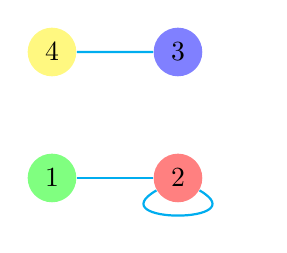
\begin{tikzpicture}
  [scale=.4,auto=left,every node/.style={circle}]
\node (n1)[fill=blue!50] at (4,4) {3};
  \node (n2)[fill=green!50] at (0,0)  {1};
  \node (n3)[fill=red!50] at (4,0)  {2};
  \node (n4)[fill=yellow!50] at (0,4)  {4};;
 \foreach \from/\to in {n3/n2,n1/n4}
    \draw[cyan,thick] (\from) -- (\to);
  \draw[cyan,thick]
  (n3) to[out=210,in=330,looseness=4] (n3);
\end{tikzpicture}
\caption{ Graph for Cube 1}\label{22g1}
\end{center}
\end{figure}

Similarly we can draw the graphs for each of the cubes Figures \ref{22g2}, \ref{22g3} and \ref{22g4}.

\begin{figure}[h]
\begin{center}
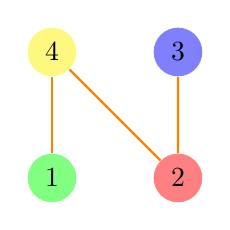
\begin{tikzpicture}
  [scale=.4,auto=left,every node/.style={circle}]
 \node (n1)[fill=blue!50] at (4,4) {3};
  \node (n2)[fill=green!50] at (0,0)  {1};
  \node (n3)[fill=red!50] at (4,0)  {2};
  \node (n4)[fill=yellow!50] at (0,4)  {4};

 \foreach \from/\to in {n3/n1,n3/n4,n2/n4}
    \draw[orange,thick] (\from) -- (\to);
\end{tikzpicture}
\caption{ Graph for Cube 2}\label{22g2}
\end{center}
\end{figure}

\begin{figure}[h]
\begin{center}
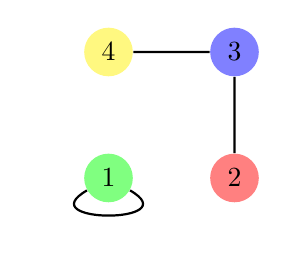
\begin{tikzpicture}
  [scale=.4,auto=left,every node/.style={circle}]
\node (n1)[fill=blue!50] at (4,4) {3};
  \node (n2)[fill=green!50] at (0,0)  {1};
  \node (n3)[fill=red!50] at (4,0)  {2};
  \node (n4)[fill=yellow!50] at (0,4)  {4};

 \foreach \from/\to in {n3/n1,n1/n4}
    \draw[black,thick] (\from) -- (\to);
     \draw[black,thick]
  (n2) to[out=210,in=330,looseness=4] (n2);
\end{tikzpicture}
\caption{ Graph for Cube 3}\label{22g3}
\end{center}
\end{figure}

\begin{figure}[h]
\begin{center}
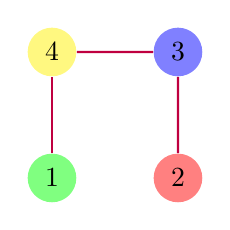
\begin{tikzpicture}
  [scale=.4,auto=left,every node/.style={circle}]
\node (n1)[fill=blue!50] at (4,4) {3};
  \node (n2)[fill=green!50] at (0,0)  {1};
  \node (n3)[fill=red!50] at (4,0)  {2};
  \node (n4)[fill=yellow!50] at (0,4)  {4};
 \foreach \from/\to in {n3/n1,n1/n4,n2/n4}
    \draw[purple,thick] (\from) -- (\to);

\end{tikzpicture}
\caption{ Graph for Cube 4}\label{22g4}
\end{center}
\end{figure}

Now combining all these graphs in a single graph, we get a graph (looks complicated) Figure \ref{22g5}.

\begin{figure}[h]
\begin{center}
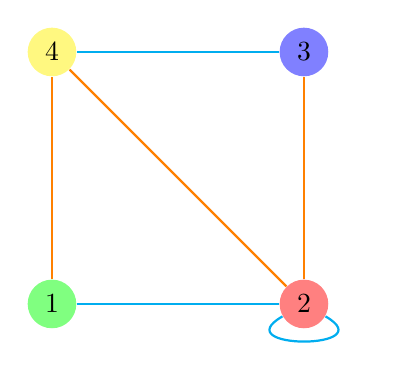
\begin{tikzpicture}
  [scale=.8,auto=left,every node/.style={circle}]
\node (n1)[fill=blue!50] at (4,4) {3};
  \node (n2)[fill=green!50] at (0,0)  {1};
  \node (n3)[fill=red!50] at (4,0)  {2};
  \node (n4)[fill=yellow!50] at (0,4)  {4};

 \foreach \from/\to in {n3/n2,n1/n4}
    \draw[cyan,thick] (\from) -- (\to);
  \draw[cyan,thick]
  (n3) to[out=210,in=330,looseness=4] (n3);
 \foreach \from/\to in {n3/n1,n3/n4,n2/n4}
    \draw[orange,thick] (\from) -- (\to); 

   
\end{tikzpicture}
\caption{ Graph for all the cubes}\label{22g5}
\end{center}
\end{figure}

